\begin{figure}[H]
    \centering
    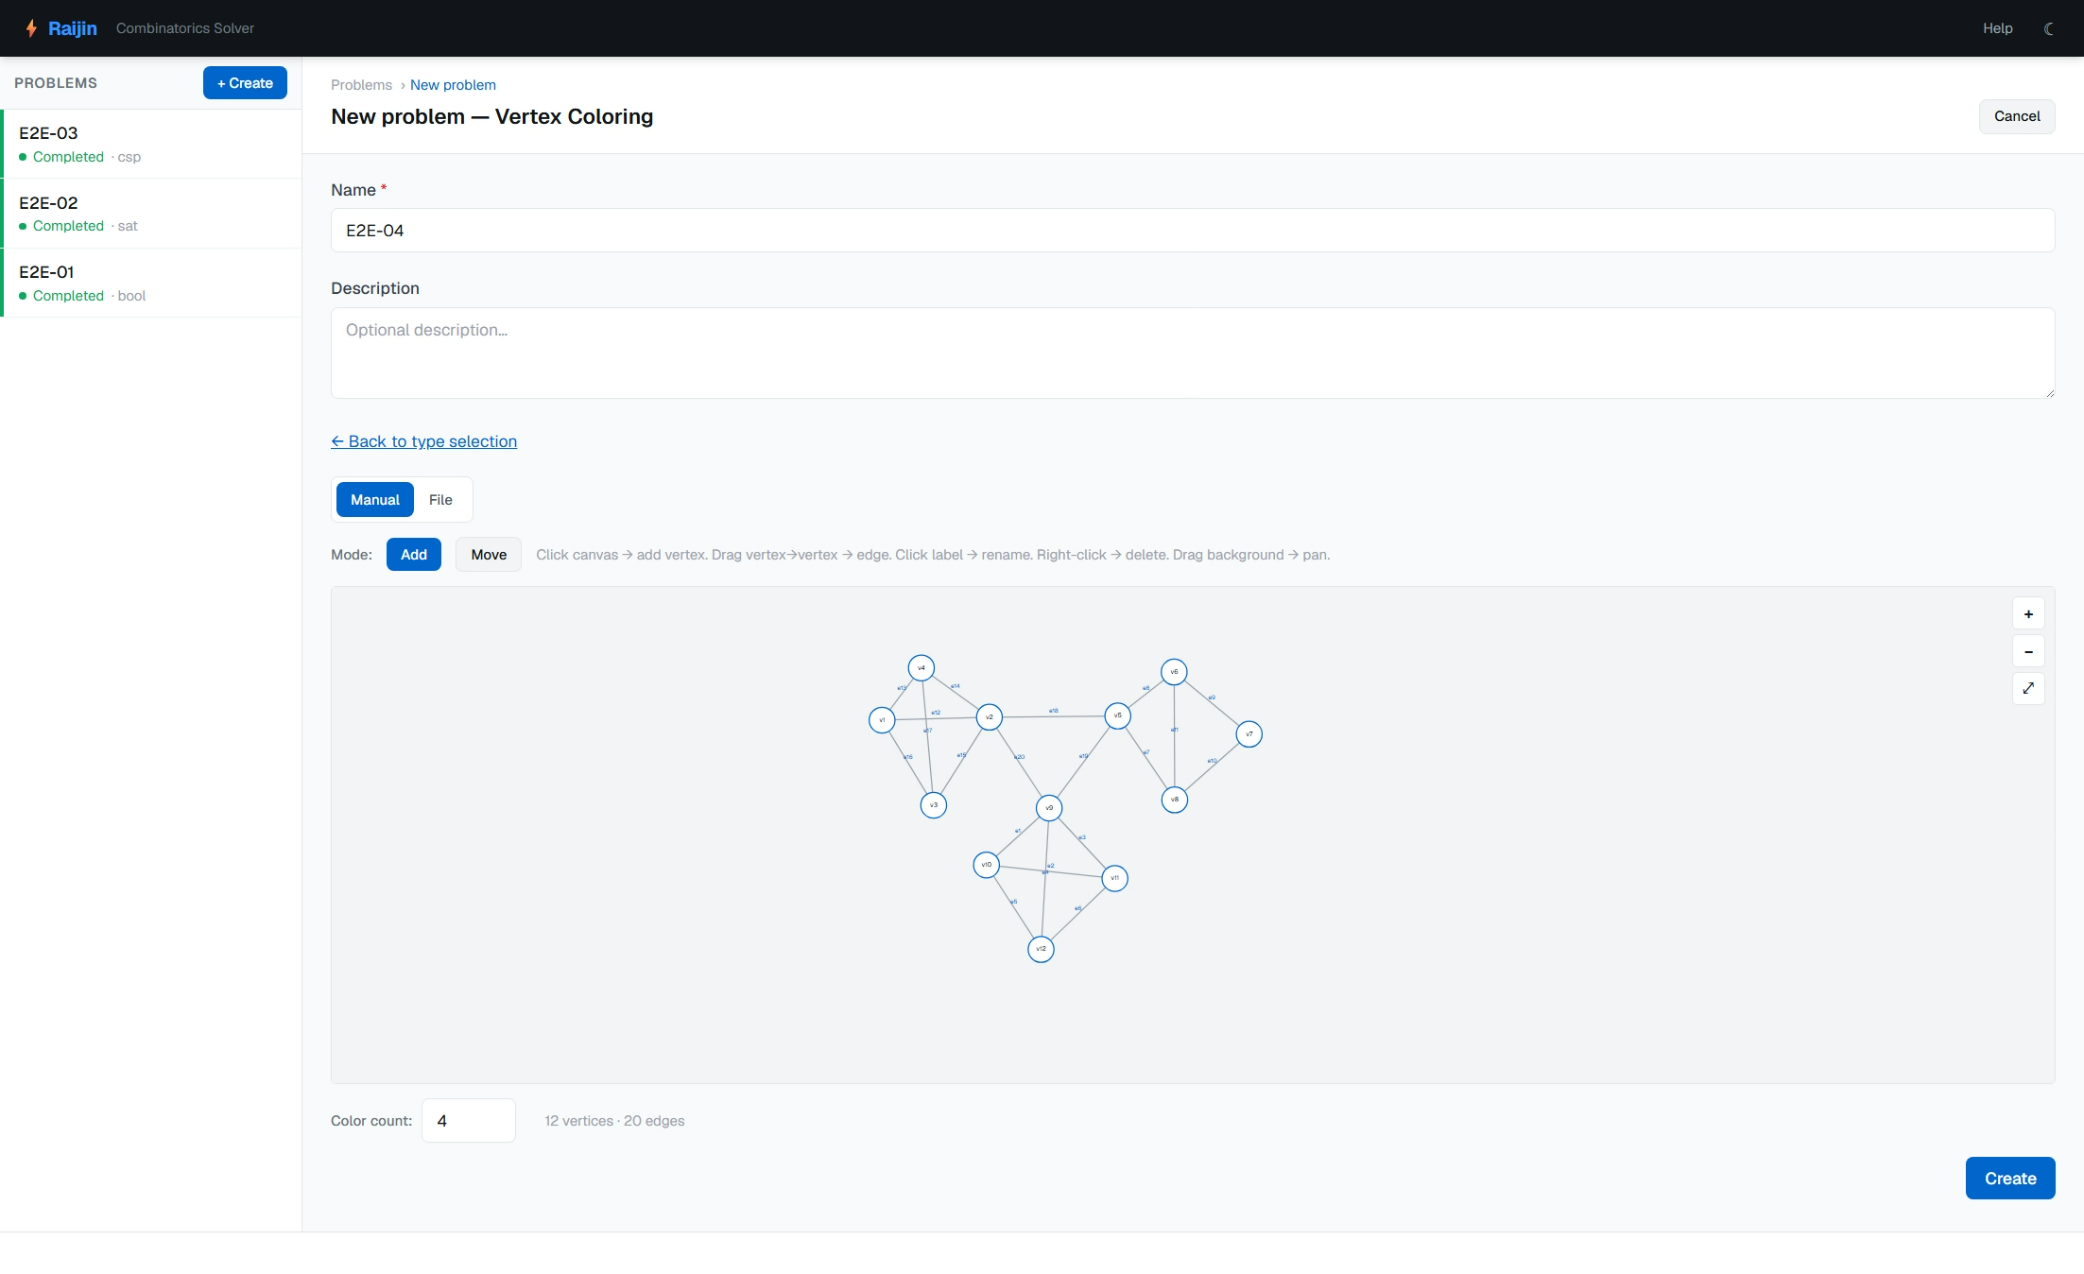
\includegraphics[width=\textwidth]{img/e2e-04-1.png}
    \caption{E2E-04 \ref{sec:testing:e2e-04}: Zadanie grafu na vrcholové farbenie (počet farieb je 4)}
    \label{fig:e2e-04-01}
\end{figure}

\begin{figure}[H]
    \centering
    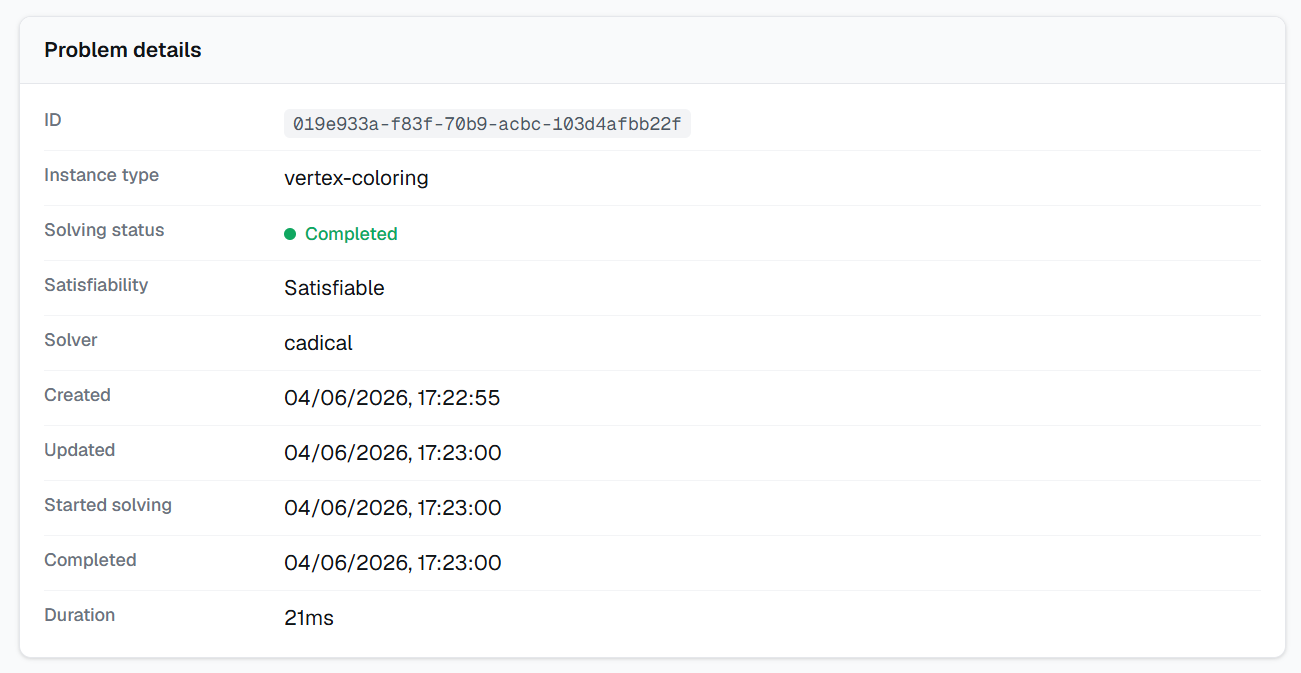
\includegraphics[width=\textwidth]{img/e2e-04-1.1.png}
    \caption{E2E-04 \ref{sec:testing:e2e-04}: Detail problému vrcholového farbenia grafu}
    \label{fig:e2e-04-02}
\end{figure}

\begin{figure}[H]
    \centering
    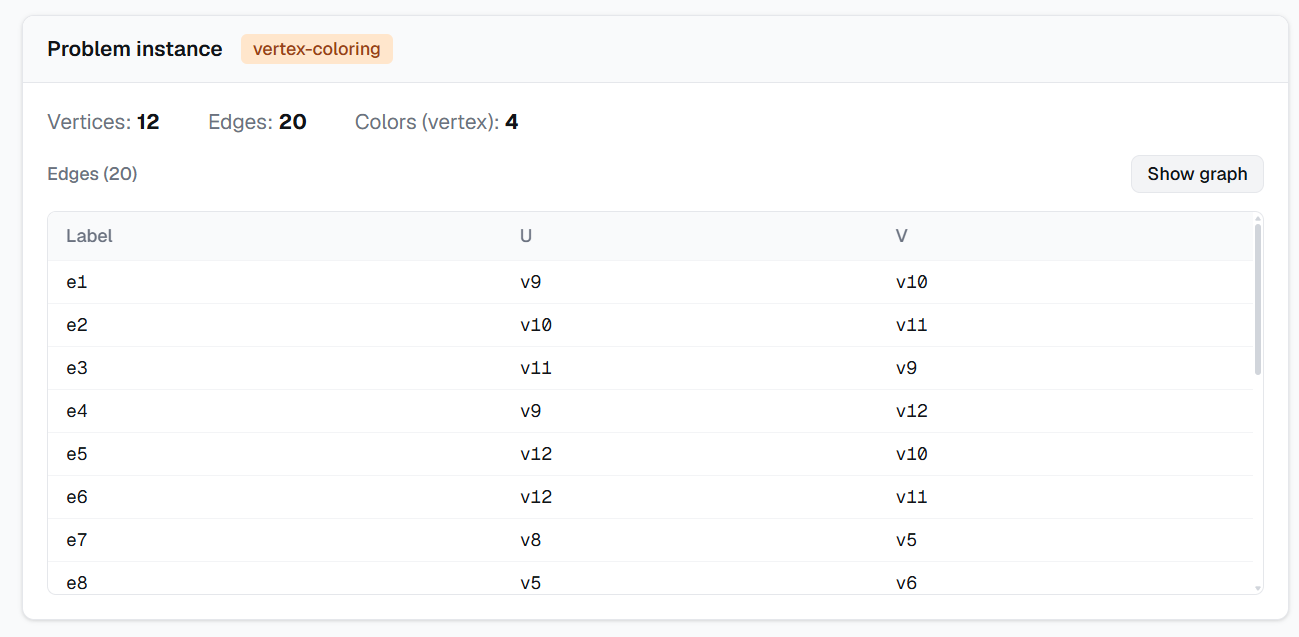
\includegraphics[width=\textwidth]{img/e2e-04-2.1.png}
    \caption{E2E-04 \ref{sec:testing:e2e-04}: Začiatok inštancie problému vrcholového farbenia grafu}
    \label{fig:e2e-04-02-01}
\end{figure}

\begin{figure}[H]
    \centering
    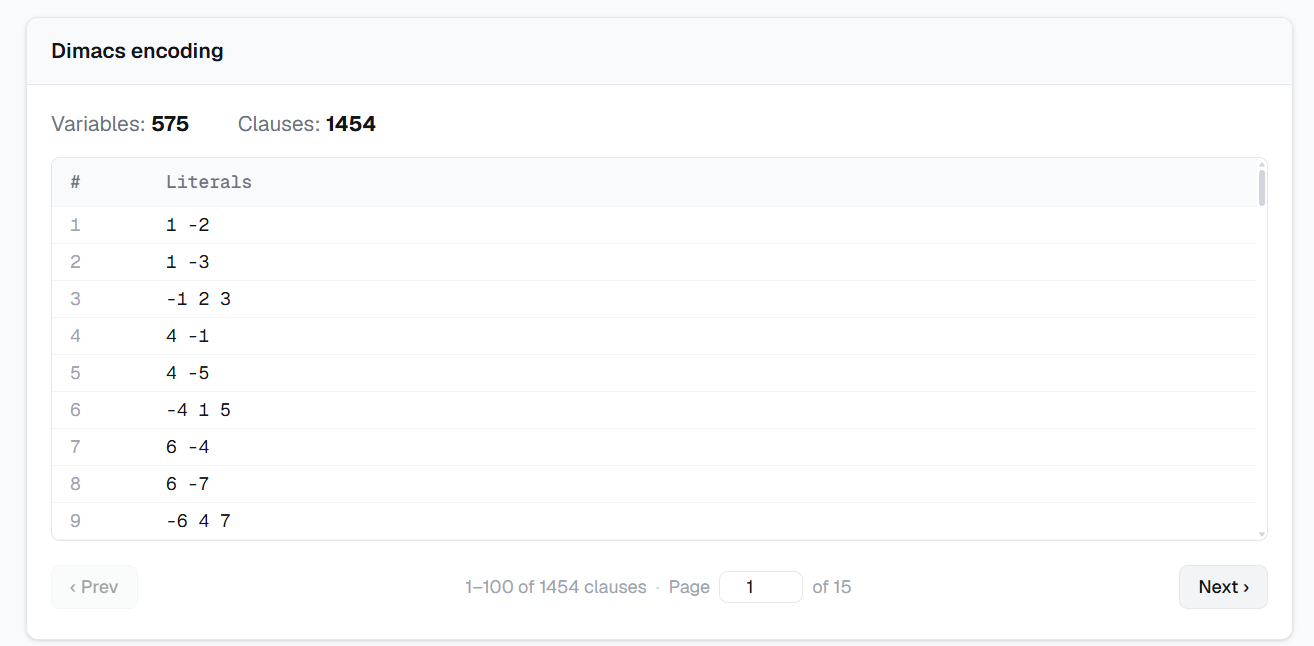
\includegraphics[width=\textwidth]{img/e2e-04-3.1.png}
    \caption{E2E-04 \ref{sec:testing:e2e-04}: Začiatok DIMACS kódovania problému vrcholového farbenia grafu}
    \label{fig:e2e-04-03-01}
\end{figure}

\begin{figure}[H]
    \centering
    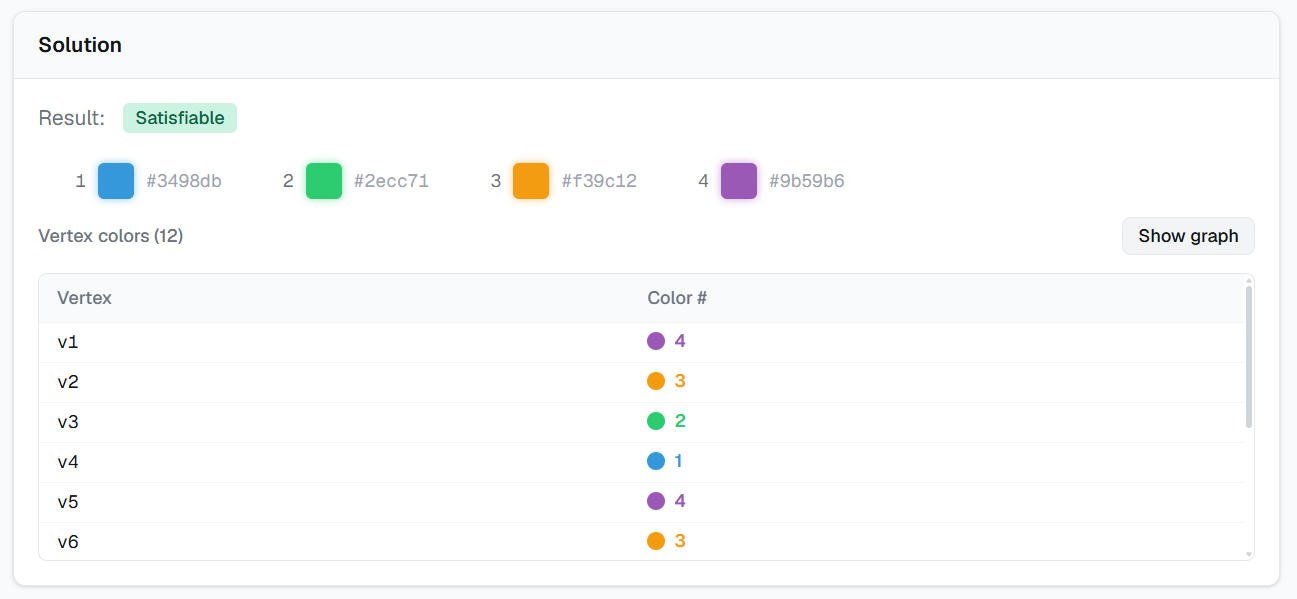
\includegraphics[width=\textwidth]{img/e2e-04-4.1.png}
    \caption{E2E-04 \ref{sec:testing:e2e-04}: Začiatok riešenia problému vrcholového farbenia grafu}
    \label{fig:e2e-04-04-01}
\end{figure}

\begin{figure}[H]
    \centering
    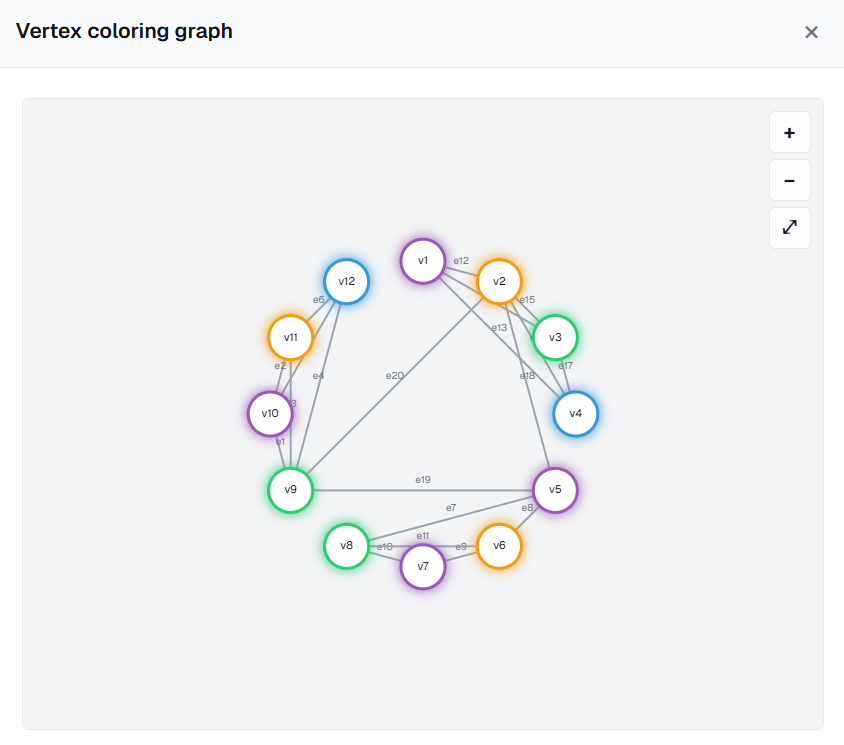
\includegraphics[width=\textwidth]{img/e2e-04-5.png}
    \caption{E2E-04 \ref{sec:testing:e2e-04}: Vizualizácia riešenia problému vrcholového farbenia grafu}
    \label{fig:e2e-04-05}
\end{figure}
